\documentclass[a4paper,12pt]{article}

% Packages (kept identical to the previous update so the build environment matches)
\usepackage{graphicx}
\usepackage{amsmath}
\usepackage{geometry}
\usepackage{fancyhdr}
\usepackage{setspace}
\usepackage{titlesec}
\usepackage{url}
\usepackage{hyperref}
\usepackage{comment}
\usepackage[most]{tcolorbox}
\usepackage{listings}
\usepackage{xcolor}
\usepackage{booktabs}
\usepackage{tabularx}
\usepackage{tikz}                  % small inline diagrams
\usetikzlibrary{positioning, arrows.meta, shapes.geometric}

\geometry{margin=0.9in}
\setstretch{1.35}

% Header and Footer
\pagestyle{fancy}
\fancyhf{}
\fancyhead[L]{Progress Report}
\fancyhead[R]{
\includegraphics[width=0.1\textwidth]{Images/IOS_Tokyo.png} \thepage }

% Title Formatting
\titleformat{\section}{\normalfont\Large\bfseries}{\thesection}{1em}{}

% Listings style (matches prior update)
\lstset{
  basicstyle=\ttfamily\small,
  breaklines=true,
  frame=single,
  numbers=left,
  numberstyle=\tiny,
  keywordstyle=\color{blue!60!black},
  commentstyle=\color{green!40!black},
  stringstyle=\color{orange!60!black}
}

% Cover Page
\title{
    \vspace{2cm}
    
\includegraphics[width=0.55\textheight]{Images/IOS_Tokyo.png} \\
    \vspace{1cm}
    \textbf{\Huge NakamuLab Progress Report} \\
    \vspace{1cm}
    \large March 2026 to April 2026 \\
    \vspace{0.5cm}

    
\includegraphics[width=0.2\textwidth]{Images/NakamuLab_logo_txt.png}
}
\author{Armando Benavidez Jr.}
\date{}

\begin{document}

% Title Page
\maketitle
\thispagestyle{empty}
\newpage

% No table of contents for this short append; the previous update already
% covers the main project structure.
\setcounter{page}{1}

% ==========================================================
% NEW SECTION: March--April Update
% ==========================================================
\section{(March to April Update) From scripts to a small visualization stack}

\tcbset{
  colback=gray!5,
  colframe=gray!40,
  boxrule=0.5pt,
  sharp corners,
  enhanced,
  fonttitle=\bfseries
}

\subsection{Project expansion and directive}
The original goal of the project was to automate the Metashape photomosaic step so that field surveys could be processed in batch instead of one at a time in the GUI. That part is now stable and working.

In this period the project has grown into a small visualization stack. The new goal is to take the outputs from Metashape (orthomosaics, JPEG previews, and optional 3D models) and serve them inside the lab on a 3D web globe so that they can be reviewed alongside a Japanese land use map. The lab can now open a browser, load all surveys at once, toggle layers on and off, and fly the camera to any survey area. The same stack also supports a simple ``Pepper's Ghost'' mode for the holographic prism display.

\begin{tcolorbox}[title=What the directive now covers]
\begin{itemize}
    \item Batch photogrammetry (already in place from the previous update).
    \item A post-processing pipeline that converts Metashape outputs into web-friendly formats (Cloud Optimized GeoTIFF, GeoJSON, glTF / 3D Tiles).
    \item Three browser viewers built on CesiumJS that read a single \texttt{manifest.json} to know which layers exist.
    \item On-premise hosting through Docker so that the same stack runs the same way on any lab machine.
\end{itemize}
\end{tcolorbox}

\subsection{Completed}
\begin{itemize}
    \item Wrote \texttt{cesium\_pipeline.py}, the post-processing script that turns the Metashape outputs into a manifest plus tiled assets.
    \item Built three viewers: a full viewer (orthos, land use, and 3D models), an ortho-only viewer, and a land use only viewer.
    \item Added a Docker setup with two services so the lab can run the full stack with one command.
    \item Wrote a project guide file (\texttt{CLAUDE.md}) so that future work using Claude Code starts with the right context already loaded.
    \item Generated an internal architecture folder (\texttt{docs/architecture/}) with one SVG per subsystem, plus a code reuse and dead code report (\texttt{docs/REPORT\_code\_duplication.md}).
\end{itemize}

\subsection{In Progress}
\begin{itemize}
    \item Cleaning up older script versions that have been superseded by \texttt{Batch\_metashape.py}. The duplication report flagged about 20 percent of the repo as deletable old versions.
    \item Aligning the land use category labels between the two viewers; a small inconsistency was found and is being fixed by generating the legend from the Python source rather than hard-coding it twice.
    \item Researching how to attach Unity to Claude Code so that future scenes built in Unity can be edited and tested with the same assistant workflow already used for the Python and Cesium parts.
\end{itemize}

\subsection{High level overview}
The diagram below shows how the pieces fit together at a glance.

\begin{center}
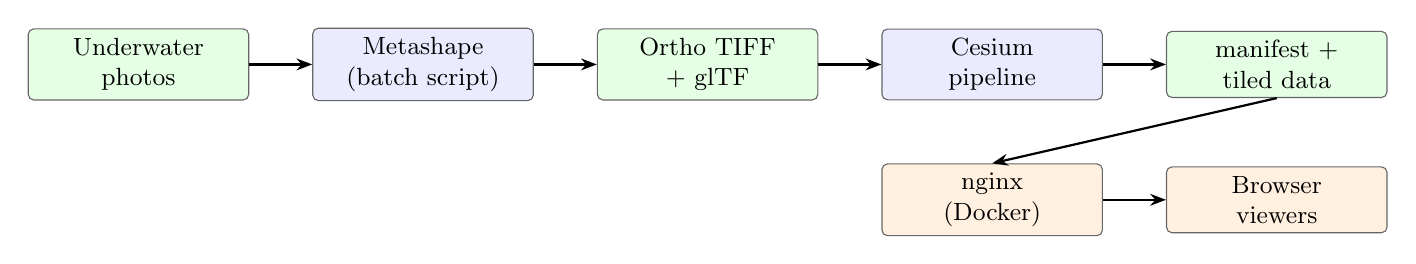
\begin{tikzpicture}[
    node distance=8mm,
    box/.style={rectangle, rounded corners=2pt, draw=black!60, fill=blue!8,
                minimum width=28mm, minimum height=8mm, font=\small, align=center},
    data/.style={rectangle, rounded corners=2pt, draw=black!60, fill=green!10,
                 minimum width=28mm, minimum height=8mm, font=\small, align=center},
    ext/.style={rectangle, rounded corners=2pt, draw=black!60, fill=orange!12,
                minimum width=28mm, minimum height=8mm, font=\small, align=center},
    arr/.style={-{Stealth[length=2mm]}, thick}
]
    \node[data] (photos) {Underwater\\photos};
    \node[box,  right=of photos] (meta) {Metashape\\(batch script)};
    \node[data, right=of meta] (out)   {Ortho TIFF\\+ glTF};
    \node[box,  right=of out] (cpipe)  {Cesium\\pipeline};
    \node[data, right=of cpipe] (man)  {manifest +\\tiled data};
    \node[ext,  below=of cpipe] (nginx) {nginx\\(Docker)};
    \node[ext,  right=of nginx] (browser) {Browser\\viewers};

    \draw[arr] (photos) -- (meta);
    \draw[arr] (meta) -- (out);
    \draw[arr] (out) -- (cpipe);
    \draw[arr] (cpipe) -- (man);
    \draw[arr] (man.south) -- (nginx.north);
    \draw[arr] (nginx) -- (browser);
\end{tikzpicture}
\end{center}

\newpage

% ==========================================================
% Docker explanation + proxy snippets
% ==========================================================
\section{Docker and the campus proxy}

\subsection{Why Docker for this project}
The post-processing pipeline relies on geospatial libraries (rasterio, geopandas, fiona) that are awkward to install on Windows because they depend on GDAL. Docker lets the project ship one image that already has the right versions installed, so any lab machine can run the pipeline the same way without first fixing a broken Python environment.

There are two services in \texttt{docker-compose.yml}:

\begin{tcolorbox}[title=Two services, kept simple]
\begin{itemize}
    \item \textbf{nginx}: an always-on web server that serves the viewers and the processed data on port 80. Restarts on its own if the machine reboots.
    \item \textbf{pipeline}: a one-shot container that runs \texttt{cesium\_pipeline.py} when called. It writes its output to a shared volume that nginx then reads.
\end{itemize}
\end{tcolorbox}

The day to day workflow is short:
\begin{lstlisting}[language=bash]
# Start the web server in the background
docker compose up -d nginx

# Run the data pipeline on demand (writes to the shared volume)
docker compose run --rm pipeline \
  --config /app/config/cesium_config.json --stage all
\end{lstlisting}

\subsection{Useful proxy snippets (kept here for reuse)}
The campus network requires the proxy \texttt{proxy.noc.titech.ac.jp:3128} for any outbound internet traffic. The same value needs to be set in several different places. These snippets are kept here so they can be copied directly the next time a fresh machine or container is set up.

\begin{tcolorbox}[title=Shell environment (PowerShell on Windows)]
\begin{lstlisting}[language=bash]
$env:HTTP_PROXY  = "http://proxy.noc.titech.ac.jp:3128"
$env:HTTPS_PROXY = "http://proxy.noc.titech.ac.jp:3128"
$env:NO_PROXY    = "localhost,127.0.0.1"
\end{lstlisting}
\end{tcolorbox}

\begin{tcolorbox}[title=Shell environment (bash / WSL / devcontainer)]
\begin{lstlisting}[language=bash]
export HTTP_PROXY=http://proxy.noc.titech.ac.jp:3128
export HTTPS_PROXY=http://proxy.noc.titech.ac.jp:3128
export NO_PROXY=localhost,127.0.0.1
\end{lstlisting}
\end{tcolorbox}

\begin{tcolorbox}[title=Pip and conda]
\begin{lstlisting}[language=bash]
pip install --proxy http://proxy.noc.titech.ac.jp:3128 <package>
conda config --set proxy_servers.http  http://proxy.noc.titech.ac.jp:3128
conda config --set proxy_servers.https http://proxy.noc.titech.ac.jp:3128
\end{lstlisting}
\end{tcolorbox}

\begin{tcolorbox}[title=Docker build (passing the proxy to the image)]
\begin{lstlisting}[language=bash]
docker build \
  --build-arg HTTP_PROXY=$HTTP_PROXY \
  --build-arg HTTPS_PROXY=$HTTPS_PROXY \
  -f Dockerfile.app -t neoreef-pipeline .
\end{lstlisting}
\end{tcolorbox}

\begin{tcolorbox}[title=Git (only when cloning over HTTPS through the proxy)]
\begin{lstlisting}[language=bash]
git config --global http.proxy  http://proxy.noc.titech.ac.jp:3128
git config --global https.proxy http://proxy.noc.titech.ac.jp:3128
\end{lstlisting}
\end{tcolorbox}

The \texttt{docker-compose.yml} file already forwards \texttt{HTTP\_PROXY} and \texttt{HTTPS\_PROXY} from the host into the build, so as long as the host shell has the variables set, the containers will pick them up automatically.

\newpage

% ==========================================================
% Unity research direction + Claude usage notes
% ==========================================================
\section{Future research and notes on tooling}

\subsection{Unity direct connect for Claude Code}
A new extension is being released that lets Claude Code talk to a running Unity editor in a way similar to how it already talks to VS Code and the file system. The early plan for this project is to use it as the bridge between the Cesium viewer (which is good for global context and 2D layers) and a Unity scene (which is better for close-up coral inspection and possible VR walkthroughs). This is a research direction, not a commitment yet, and a separate report will be written once the extension is installed and tested.

The first questions to answer are:
\begin{itemize}
    \item Can the same glTF and 3D Tiles outputs that the Cesium pipeline already produces be loaded directly into Unity, or does an extra conversion step need to be added?
    \item Can Claude Code drive simple Unity tasks (load a model, set lighting, place a camera) through the extension, in the same way it currently edits Python files?
    \item What does this add for the lab in practice (close-up viewing, VR, Pepper's Ghost on a different display) that the current Cesium viewer does not already cover?
\end{itemize}

\subsection{Working with Claude during this period}
A few small habits made the work with Claude Code noticeably easier and are worth recording for the next person on the project.

\begin{tcolorbox}[title=Project context lives in CLAUDE.md]
A file named \texttt{CLAUDE.md} at the repo root is read automatically when Claude Code is opened in this folder. It captures the tech stack, the folder layout, the run commands, and the rules of the project (for example: never commit \texttt{cesium\_config.json}, two different Dockerfiles exist, the proxy is needed on campus). Writing it once saves explaining the same things at the start of every session.
\end{tcolorbox}

\begin{tcolorbox}[title=Reports as .md files instead of long chat answers]
For anything that is more than a small change, asking for the answer as a markdown file in \texttt{docs/} works better than a long reply in the chat. The duplication report and the architecture SVGs were both produced this way and now live in the repo where the rest of the lab can read them later.
\end{tcolorbox}

\begin{tcolorbox}[title=Memory across sessions]
Claude can keep short notes between sessions (for example, the user role, project preferences, and known issues such as the leaked token in \texttt{cesium\_config.json}). This means that the second and third sessions on a topic skip a lot of repeat context and start closer to where the last one ended.
\end{tcolorbox}

\begin{tcolorbox}[title=Small, named changes work better than ``do everything'']
Asking Claude to do one named thing at a time (``write the duplication report'', ``add the SVG folder'', ``draft the April update'') gave cleaner results than asking for a broad list at once. The list still happened, but as separate steps that could be reviewed one by one.
\end{tcolorbox}

\subsection{In Summary}
This period moved the project from a working batch script to a small in-house visualization stack that the lab can open in a browser. Docker is the glue that makes the stack reproducible, and the proxy snippets above will save time the next time a fresh machine is set up. The next two periods will focus on the cleanup tasks flagged in the duplication report, deciding whether the Unity bridge is worth pursuing, and continuing to write project knowledge into the repo so the next person can pick it up without a long handover.

\end{document}
